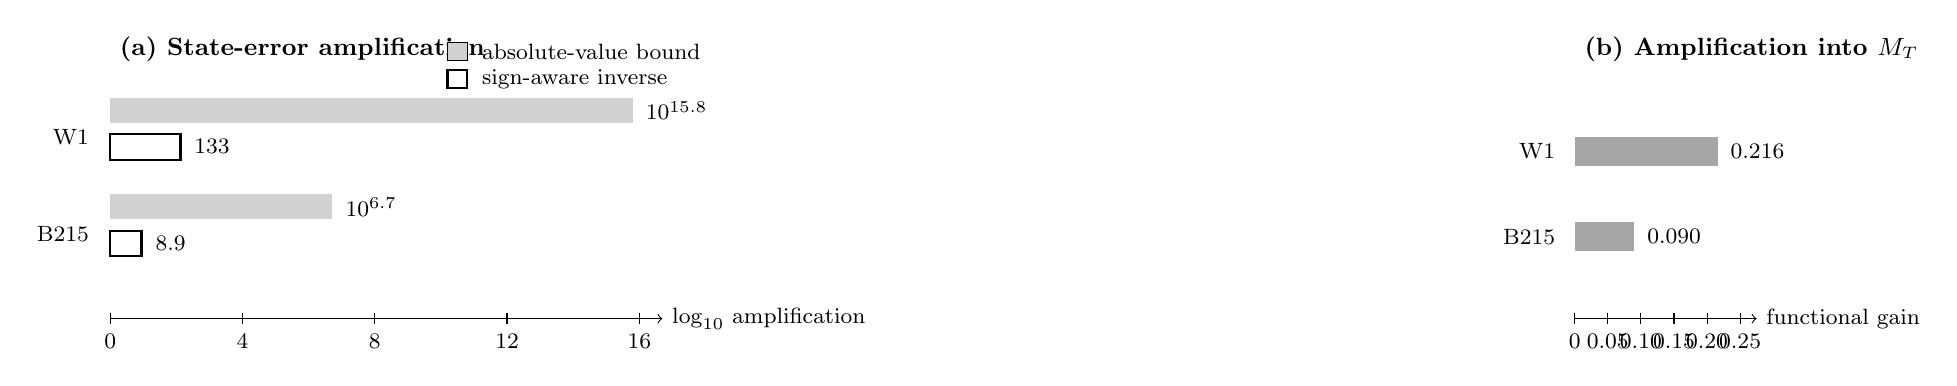
\begin{tikzpicture}[x=0.42cm,y=0.72cm,every node/.style={font=\footnotesize}]
  % Left panel: log10 amplification
  \node[anchor=west,font=\small\bfseries] at (0,5.2)
    {(a) State-error amplification};

  \draw[->] (0,0.45) -- (16.7,0.45)
    node[anchor=west] {\(\log_{10}\) amplification};
  \foreach \x in {0,4,8,12,16} {
    \draw (\x,0.35)--(\x,0.55);
    \node[below] at (\x,0.35) {\x};
  }

  \node[anchor=east] at (-0.35,3.65) {W1};
  \node[anchor=east] at (-0.35,1.95) {B215};

  % W1
  \fill[black!18] (0,3.9) rectangle (15.8,4.35);
  \draw[thick] (0,3.25) rectangle (2.124,3.70);
  \node[anchor=west] at (15.9,4.12) {\(10^{15.8}\)};
  \node[anchor=west] at (2.25,3.48) {\(133\)};

  % B215
  \fill[black!18] (0,2.2) rectangle (6.7,2.65);
  \draw[thick] (0,1.55) rectangle (0.949,2.00);
  \node[anchor=west] at (6.82,2.42) {\(10^{6.7}\)};
  \node[anchor=west] at (1.08,1.78) {\(8.9\)};

  \draw[fill=black!18] (10.2,5.0) rectangle (10.8,5.32);
  \node[anchor=west] at (10.95,5.16) {absolute-value bound};
  \draw[thick] (10.2,4.52) rectangle (10.8,4.84);
  \node[anchor=west] at (10.95,4.68) {sign-aware inverse};

  % Right panel: functional amplification
  \begin{scope}[xshift=18.6cm]
    \node[anchor=west,font=\small\bfseries] at (0,5.2)
      {(b) Amplification into \(M_T\)};

    \draw[->] (0,0.45) -- (5.5,0.45)
      node[anchor=west] {functional gain};
    \foreach \x/\lab in {0/0,1/0.05,2/0.10,3/0.15,4/0.20,5/0.25} {
      \draw (\x,0.35)--(\x,0.55);
      \node[below] at (\x,0.35) {\lab};
    }

    \node[anchor=east] at (-0.3,3.4) {W1};
    \node[anchor=east] at (-0.3,1.9) {B215};

    \fill[black!35] (0,3.15) rectangle (4.32,3.65);
    \fill[black!35] (0,1.65) rectangle (1.80,2.15);

    \node[anchor=west] at (4.42,3.40) {\(0.216\)};
    \node[anchor=west] at (1.90,1.90) {\(0.090\)};
  \end{scope}
\end{tikzpicture}
